\section{Ablation studies on the effect of hyperparameters}
In this section, we present results of the ablation studies on the effect of hyper parameters $\tau$ and $\gamma$. The paper \cite{helwegen2019latent} considers a binary convolutional architecture called \textit{BVGG} net as given in \cite{simonyan2014very} inspired from the architecture of ConvNet in \cite{courbariaux2016binarized} we discussed before. The authors have shown that the main action which matters for BOP is flipping weights. The question boils down to the following: based on a sequence of gradients, whether to flip a weight or not. BOP should pay attention to the consistency and the strength (absolute value) of the gradient signals. In BOP the consistent signal is selected by looking at exponential moving average of gradients.
\begin{equation}
    m_t=(1-\gamma)m_{t-1} + \gamma g_t=\gamma \sum_{r=0}^{t}(1-\gamma)^{(t-r)}g_r \label{eqn:gamma}
\end{equation}
where $g_t$ is the gradient at time $t$, $m_t$ is exponential moving average and $\gamma$ is the adaptivity rate. The weight flip is determined by comparing the moving average with a threshold called $\tau$:
\begin{equation}
    w_t^i =
    \begin{cases*}
      -w_{t-1}^i & if $|m_t^i|\geq\tau$ and sign$(m_t^i)$ = sign$(m_{t-1}^i)$ \\
      w_{t-1}^i        & otherwise \label{eqn:tau}
    \end{cases*}
\end{equation}
The two hyper parameter for BOP are $\tau$ and $\gamma$. In this section we show the results of the experiments on BVGG net with BOP as optimization method and with CIFAR10 dataset. To use the dataset for training a binary network, in our work similar modifications are done to the dataset as \cite{helwegen2019latent}. We use batch normalization to normalize the activations with a minibatch size of $64$. 

A non zero threshold $\gamma$ avoids rapid flip of weights when the gradient reverses on a weight flip. One thing to note here is that high value of $\tau$ can result in never flipping weights even though there is pressure from a consistent gradient signal. As given in the paper, a higher adaptivity rate $\gamma$ gives more adaptive moving average which implies that if a new gradient signal pressurizes a weight to flip, it take lesser time steps to do so.

\begin{figure}[!ht]
\centering
    \begin{subfigure}{0.98\textwidth}
        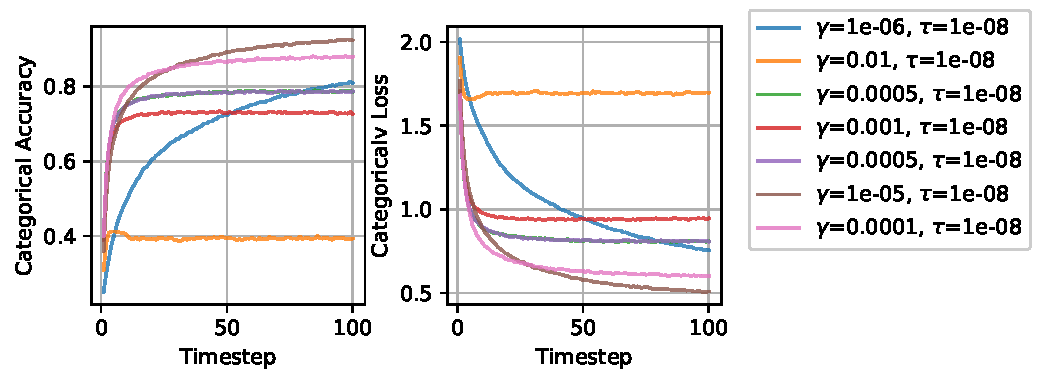
\includegraphics[width=1.\linewidth]{fig/AccuracyLossBNfixedtau.pdf}
        \caption{Fixed $\tau$}
        \label{fig:bnfixedtau}
    \end{subfigure}
    \begin{subfigure}{0.98\textwidth}
        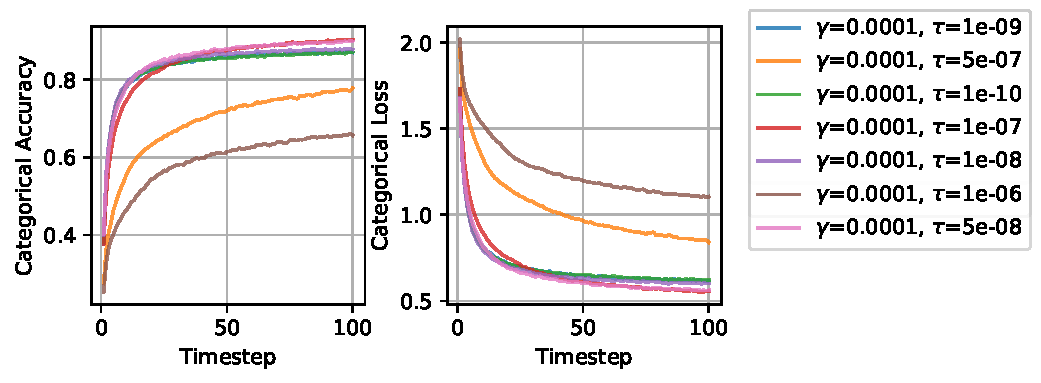
\includegraphics[width=1.\linewidth]{fig/AccuracyLossBNfixedgamma.pdf}
        \caption{Fixed $\gamma$}
        \label{fig:bnfixedgamma}
    \end{subfigure}
    \caption{Ablation studies for $\tau$ and $\gamma$ for Batch Normalization}
\end{figure}

Keeping $\tau$ same ($10^{-8}$) we see the effect of different $\gamma$ in Fig (\ref{fig:bnfixedtau}). From eq (\ref{eqn:gamma}) it is clear that with the increase in the value of $\gamma$, $m_t$ fluctuates more. A high $\gamma (=0.01)$ gives very poor performance as high adaptivity rate makes weight to flip in less time steps if a gradient signal starts pressurizing it. Even though in the very beginning of the training, the accuracy trend is steep in case of $\gamma=0.01$, within a short period of time the accuracy converges to $40\%$. A low $\gamma (=10^{-6})$ provides stable training process but it takes long time to fully converge to final accuracy. From the plots we found for $\tau=10^{-8}$, $\gamma=10^{-5}$ performs best and converges to training accuracy $92.15\%$.

Fig (\ref{fig:bnfixedgamma}) gives training accuracy and loss for different threshold $\tau$ and a fixed $\gamma(=0.0001)$. As explained in the paper, $\tau$ should be a non zero real number but not so big that the weight flipping is hindered. In our simulation result, networks with $\tau$ in the range of $10^{-8}$ perform nearly same. 



\section{Layer Normalization}
Till date in most of the works in the line of BNN, batch normalization is used between consecutive non-linear layers in order to stabilize the training. The aim of batch normalization is to normalize the inputs with the global mean and variance but calculating mean and variance of activations for the whole dataset is very costly. So batch normalization is done in small batches and the estimated mean and variances vary from one minibatch to other. The main challenge of using batch normalization is limitation in batch size.
\begin{figure}[!ht]
    \centering
    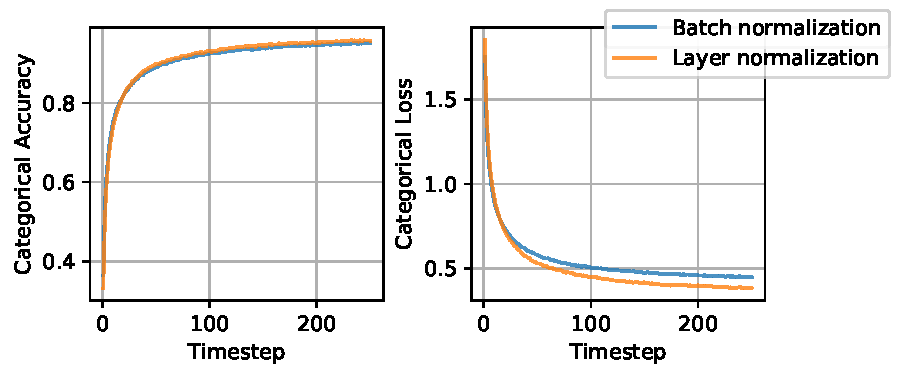
\includegraphics[scale=0.8]{fig/AccuracyLosscompareBNLN.pdf}
    \caption{Comparison of BN and LN with $\tau=10^{-8}$ and $\gamma=10^{-5}$ in Binary VGG net with CIFAR10 dataset and BOP optimizer}
    \label{fig:bnln}
\end{figure}
If the batch size is very small the variance of the estimates would be very high which makes it difficult to use batchnorm in online learning. Also in case of recurrent neural network, use of batchnorm is difficult as the layer statistics change at each timestep. In this section, we look into layer normalization as an alternative solution to avoid these problems \cite{lei2016layer}. 

\begin{figure}[!ht]
\centering
    \begin{subfigure}{0.98\textwidth}
        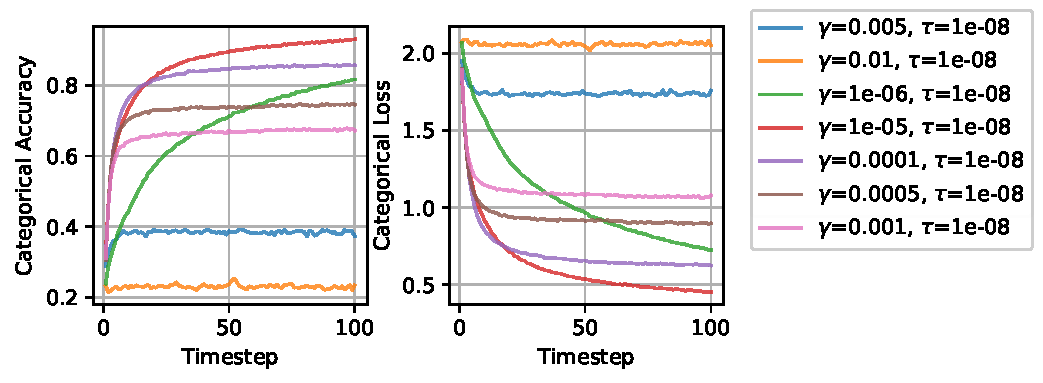
\includegraphics[width=1.\linewidth]{fig/AccuracyLossLNfixedtau.pdf}
        \caption{Fixed $\tau$}
        \label{lnfixedtau}
    \end{subfigure}
    \begin{subfigure}{0.98\textwidth}
        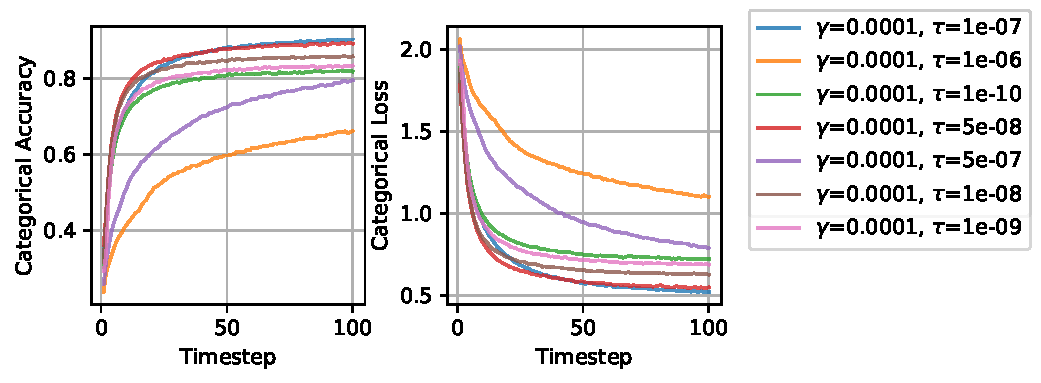
\includegraphics[width=1.\linewidth]{fig/AccuracyLossLNfixedgamma.pdf}
        \caption{Fixed $\gamma$}
        \label{lnfixedgamma}
    \end{subfigure}
    \caption{Ablation studies for $\gamma$ and $\tau$ for layer normalization} \label{fig:ln_ablation}
\end{figure}

Layer normalization works by normalizing across the activation (features) passed between two consecutive layers instead of over a mini batch. In layer normalization, the statistics are calculated across each feature and are independent of other example. We propose to use layer normalization instead of batch normalization as an alternate way of stabilizing training. In Fig \ref{fig:bnln}, we provide a comparison of training performances of layer normalization and batch normalization for $\tau=10^{-8}$ and $\gamma=10^{-5}$. It is clear that layer normalization performs slightly better than batch normalization for this choice of hyper parameter. 


In Fig. \ref{fig:ln_ablation}, we provide a comprehensive ablation study for the effect of hyper parameters of BOP in conjuction with layer normalization. From Fig (\ref{lnfixedtau}), we can observe that for fixed $\tau(=10^{-8})$ the performance of BVGG net is best for $\gamma=10^{-5}$ and the explanation follows from the batch normalization ablation studies. Similarly, as shown in Fig (\ref{lnfixedgamma}) for fixed $\gamma$, $\tau$ in the range of $10^{-8}$ has nearly same performance.

The above studies conclude that layer normalization can be used as a viable alternative to Batch Normalization in the case of training Binary Neural Networks. This can be especially useful in the cases where BNN has to be trained in an online fashion (as in the case of deep reinforcement learning) where acquiring a mini-batch of sufficient size to alleviate the affect of noise variance in estimation is either costly or undesirable.

  
  




